%!TEX root = ../lections.tex
\newcommand{\R}{\mathbb{R}}
\newcommand{\Z}{\mathbb{Z}}
\section{Общие закономерности теории колебаний} % (fold)

Колебательные процессы и системы настолько широко распространены в
природе, технике и обществе, что любой из нас с ними неоднократно
сталкивается в повседневной жизни и, по-видимому, без труда сформулирует
основные их свойства. Действительно, когда мы слышим о колебаниях
температуры, курса валют, электрического напряжения, маятника, уровня воды
и так далее, нам понятно, что речь идет о процессах во времени или в
пространстве, обладающих той или иной степенью повторяемости и
возвращаемости к начальному или близкому состояниям. Причем, эти базовые
свойства процессов не зависят от природы систем и поэтому могут быть
описаны и изучены с единой точки зрения в рамках общего
междисциплинарного подхода. Именно такой подход и развивает теория
колебаний, предметом которой являются колебательные явления и процессы в
системах различной природы. Колебательные свойства реальных систем теория
колебаний получает из анализа соответствующих моделей. В результате такого
анализа устанавливается связь между параметрами модели и её
колебательными свойствами.

Теория колебаний является как прикладной, так и фундаментальной
наукой. Прикладной характер теории колебаний определяется её
многочисленными приложениями в физике, механике, автоматическом
управлении, радиотехнике и электронике, приборостроении и т.д. В этих
областях науки методами теории колебаний проведено исследование большого
числа различных систем и явлений. Более того, на базе теории колебаний
возникли новые технические направления – вибротехника, вибродиагностика,
биомеханика и др. Фундаментальный характер теории колебаний заключен в
самих моделях, которые она изучает. Это так называемые динамические
системы, с помощью которых можно описать любую детерминированную`'
эволюцию во времени или во времени и пространстве. Именно изучение
динамических систем позволило теории колебаний ввести понятия и
положения, развить методы и получить результаты, оказывающие большое
влияние на другие естественные науки. Здесь достаточно отметить
линеаризованную теорию устойчивости, понятия автоколебаний и резонанса,
теорию бифуркаций, хаотические колебания и др.
% subsection общие_закономертности_теории_колебаний (end)

\section{Динамические системы} % (fold)
Рассмотрим систему, состояние которой определяется вектором $\vec x (t) 
\in \R^n$. Предположим, что эволюция системы определяется одно-параметрическим семейством операторов $G^t$, $t\in\R$ (или $t\in\R^+$) или $t\in \Z$ (или $t\in\Z^+$), таких, что состояние системы в момент $t$
\begin{equation}
	\label{eq:1.1}
	\vec x(t,\vec x_0) = G^t \vec x_0,
\end{equation}
где $\vec x_0$ -- начальное состояние (начальная точка). Предположим также, что эволюционные операторы удовлетворяют двум следующим свойствам, отражающим детерминистический характер описываемых процессов.
\begin{enumerate}
	\item $G^0$ -- тождественный оператор, т.е.
	\begin{equation}
	\label{eq:1.2}
		\vec x(0, \vec x_0), \text{ для любых } \vec x_0.
	\end{equation}

Это свойство означает, что состояние системы не может изменяться самопроизвольно.

	\item  Второе свойство эволюционных операторов имеет вид:
	\begin{equation}
		\label{eq:1.3}
		G^{t_1+t_2}= G^{t_1} \circ G^{t_2}= G^{t_2} \circ G^{t_1},
	\end{equation}
	т.е.
	\begin{equation}
		\label{eq:1.4}
		\vec x (t_1+t_2, \vec x_0) = \vec x (t_1, \vec x(t_2, \vec x_0)) = \vec x (t_2, \vec x (t_1,x_0))
	\end{equation}
\end{enumerate}
 
 Согласно \eqref{eq:1.3} система приходит в одно и то же финальное состояние независимо от того, достигается ли оно за один временной интервал $t_1+t_2$, или за несколько последовательных интервалов $t_1$ и $t_2$, суммарной равных $t_1+t_2$.

 Совокупность всех начальный точек $X$ или всех возможных состояний системы (в рассматриваемом случае $X= \R^n$) называется фазовым пространством, а пара $\qty(X,\{G^t\})$, где семейство эволюционных операторов удовлетворяют условиям \eqref{eq:1.3} - \eqref{eq:1.2}, -- динамической системой (ДС).

 ДС делятся на два важных класса -- с непрерывным временем, если $t\in \R$ или $\R_+$,  и с дискретным временем, если $t\in \Z$ или $\Z_+$.

 Эволюция системы соответствует движению изображающей точки в фазовом пространстве вдоль траектории $\Gamma = \bigcup\limits_t G^t \vec x_0$. Семейство $ \Gamma^+ = \bigcup\limits_{t\geq 0} G^t \vec x_0 $\quad  $ \qty(\Gamma^- = \bigcup\limits_{t< 0} G^t \vec x_0)$ называется положительной (отрицательной) полутраекторией, проходящей через начальную точку $\vec x_0$. Если семейство $\{G^t\}$ является непрерывным по $t$ (для ДС с непрерывным временем ), то траектории (полутраектории) представляют собой непрерывные кривые в $X$. Для ДС с дискретным временем траектории являются дискретными подмножествами в фазовом пространстве.

 Введем необходимое в дальнейшем понятие инвариантности множества.
 Множество $A \subset X$ называется положительно (отрицательно) инвариантным , если оно состоит из положительных полутраекторий, т.е. $A$ - положительно (отрицательно) инвариантно, если $G^t A \subset A, t>0 ~ (t<0)$. Множество $A$ называется инвариантным, если оно одновременно инвариантно как положительно, так и отрицательно.	


\subsection{Типы траекторий} % (fold)
\label{subsubsec:1.2.1}
Дадим определение основных типов траекторий ДС.
\begin{itemize}
	\item Точка $\vec x_0$ называется неподвижной точкой ДС, если $G^t \vec x_0 = \vec x_0$ для всех $t$ (для систем с непрерывным временем такие точки чаще называют состояниями или положениями равновесия).
	\item Точка $\vec x_0$ называется периодической, если существует такое $T>0$ , что $G^t \vec x_0 = \vec x_0$ и $G^t \vec x_0 \neq \vec x_0$ для $0<t<T$, а соответствующая траектория $\bigcup\limits_{0\leq t \leq T} G^t \vec x_0$ динамической системы, проходящая через эту точку -- периодической. Периодическая траектория является замкнутой кривой в фазовом пространстве ДС с непрерывным временем и совокупностью $T$-периодических точек для ДС с дискретным временем.
	\item Точка $\vec x_0$ называется неблуждающей, если для любой окрестности открытого множества $U \ni \vec x_0$ этой точки и любого $t_0>0$ найдется сколь угодно большое $t>t_0$, такое что $G^t U \cap U \neq \varnothing $. Траектория, проходящая через такую точку, называется неблуждающей. 
\end{itemize}

Между траекториями ДС и движениями реальных систем существует соответствие. Неподвижным точкам ДС отвечают стационарные состояния реальных систем, периодическим траекториям -- периодические движения, а неблуждающим траекториям -- движения с некоторым повторением их состояний во времени.

Заметис, что вышеприведенные траектории могут существовать и в ДС, у которых фазовое пространство не обязательно $\R^n$. Например, фазовым пространством динамической системы, описывающей колебания математического маятника является цилиндр $X= S^1 \times \R $, поскольку состояние маятника в любой момент времени однозначно описывается значением угловой переменной $\phi(t)$, определенной с точностью до $2\pi ~ (\phi \in S^1)$  значением её скорости $\dot \phi \in \R$.
% subsubsection типы_траекторий (end)

\subsection{Динамические системы с непрерывным временем} % (fold)
Для многих ДС с непрерывным временем правило, которое позволяет найти состояние в любой момент времени по начальному состоянию, задается системой обыкновенных дифференциальных уравнений
\begin{equation}
	\dot x_i = f_i (x_1,x_2,\dots, x_N), ~ i = 1,2, \dots, N
\end{equation}
или в векторной форме
\begin{equation}
	\label{eq:1.5}
	\vec {\dot x_i} = \vec F (\vec x), ~ \vec x \in \R^n, ~ \vec F: \R^n \rightarrow \R^n,
\end{equation}
для которой условия существования и единственности решений выполнены (здесь и далее мы будем обозначать точкой дифференцирование по времени). В этом случае семейство $G^t \vec x_0$ задается просто решением системы \eqref{eq:1.5} с начальным условием $\vec x(0, \vec x_0)= \vec x_0$. Например, для линейной системы
\begin{equation}
	\dot {\vec x} = A \vec x,
\end{equation} 
где $A$ -- матрица размерности $n \times n $ с постоянными коэффициентами, решение имеет вид $\vec x(t, \vec x_0)= e^{At} \vec x_0$, в котором $e^{At}$ -- матрица $n \times n$. Поскольку матрицы $e^{A_1t}$ и $e^{A_2t}$ коммутируют для любой пары $t_1, t_2$, то свойство \eqref{eq:1.3}:
\begin{equation}
	e^{A(t_1+t_2)}= e^{At_1}\circ e^{At_2} = e^{At_2}\circ e^{At_1} 
\end{equation}
выполняется. Свойство \eqref{eq:1.2} также, очевидно, выполнено.

В качестве другого примера рассмотрим систему, заданную в полярных координатах
\begin{equation}
	\dot \rho = \lambda \rho, \quad \dot \phi = \omega
\end{equation}
Следовательно, эволюционные операторы задаются следующим образом
\begin{equation}
	G^t:\quad (\rho_0,\phi_0) \rightarrow (\rho_0 e^{\lambda t}, \omega t + \phi).
\end{equation}
Очевидно, что свойства \eqref{eq:1.2}-\eqref{eq:1.3} выполняются.

Обратим внимание н ато, что правая часть системы \eqref{eq:1.5} явно от времени не зависит. Такие системы называются \textbf{автономными}. Существует также большое число задач (например, системы, подверженные внешнему переменному силовому воздействие), описываемых динамическими системами, правые части которых явно зависят от времени. Они называются \textbf{неавтономными}.

% subsubsection динамические_системы_с_непреры (end)

\subsection{Динамические системы с дискретным временем} % (fold)
ДС с дискретным временем обычно определяют следующим образом
\begin{equation}
	\label{eq:1.6}
	\vec x(n+1)= \vec F (\vec x(n)),
\end{equation}
где $\vec F: ~ \R^n \rightarrow \R^n$ -- отображение и $n \in Z_+ = \{0,1,2, \dots\}$ -- дискретное время. Для таких систем траектория представляет собой конечную или счетную совокупность точек в $\R^n$. Иногда употребляют другую эквивалентную форму записи ДС с дискретным временем
\begin{equation}
	\vec {\bar {x}} = \vec F (\vec x),
\end{equation}
где $\vec{\bar x}$ является образом точки $\vec x$ под действием отображения $F$. В настоящем курсе мы будем использовать ту и другую форму записи точечных отображений.

Поясним понятие ДС с дискретным временем на примере одномерного отображения
\begin{equation}
	\label{eq:1.7}
	\bar x = 2x, \textrm{mod}\,1
\end{equation}
Фазовым пространством этого отображения является интервал $[0, 1]$. Пусть 
$x(0)= 1/5$. Непосредственно из \eqref{eq:1.7} получим
\begin{equation}
	x(0) = \frac15 \rightarrow x(1)= \frac25 \rightarrow x(2) = \frac45 \rightarrow x(3) = \frac35 \rightarrow x(4) = \frac15.	
\end{equation}
Следовательно, рассматриваемая полутраектория является периодической с периодом 4 (рис. \ref{fig:1.1}). На первый взгляд кажется, что при таком простом правиле точечного преобразования \eqref{eq:1.4} временная эволюция переменной $x(n)$ при любых начальных условиях может оказаться простой и предсказуемой. Оказывается, что это не так. Если значение $x(0$ известно не точно, а с некоторой точность $\epsilon$ , предсказать будущее поведение $x(n)$ не удается. После достаточно большого числа итераций интервал $J_{\epsilon} = \qty(x(0) 0 \epsilon, x(0) + \epsilon)$ будет покрывать всё фазовое пространство - интервал $[0, 1]$. ругими словами, существуют траектории, проходящие через начальные точки в $J_\epsilon$, растягивающие произвольный кусок фазового пространства. Непредсказуемость вызывается здесь неустойчивость траекторий. Это феномен так называемого детерминированного хаоса, когда в детерминированной системе из-за неустойчивости траекторий возникают непредсказуемые наперед движения.
 \begin{figure}[h!]
 	\centering
    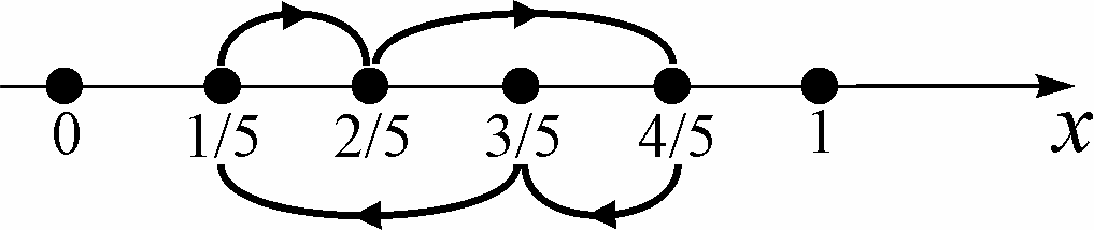
\includegraphics[]{fig/lect1/1}
 	\caption{Полутраектория системы \eqref{eq:1.4} с начальным условием $x(0)=1/5$}
 	\label{fig:1.1}
\end{figure}

% subsubsection динамические_системы_с_дискретным_временем (end)

\subsection{Динамические системы с диссипацией} % (fold)
Рассмотрим динамическую систему \eqref{eq:1.5}  и введем для неё понятие шара диссипации. Говорят, что гладкая поверхность $S=\{\phi(x) = 0 \}$ будет трансверсальной к векторному полю $\vec F (\vec x) $, если скалярное произведение
\begin{equation}
	\qty(\grad \phi(\vec x), \vec F(\vec x)) \neq 0 \qquad \forall \vec x \in S,
\end{equation}
где 
\begin{equation}
	\grad \phi(\vec x) = \qty(\pdv{\phi_1}{x_1},\pdv{\phi_2}{x_2},\dots, \pdv{\phi_m}{x_m})
\end{equation}
Если $S$ топологическая сфера, т.е. граница топологического шара $D$, то шар $D$ называется гаром диссипации, если
\begin{equation}
	\qty(\grad \phi(\vec x), \vec F(\vec x)) < 0 \qquad \forall \vec x \in S,
\end{equation}
Это означает, что векторное поле $\vec F(\vec x)$ на $S$ ориентировано внутрь $D$ (рис. \ref{fig:1.2}). Очевидно, что траектории, входящие в $D$, остаются в нем навсегда. Такие динамические системы называются диссипативными. Наибольшее внимание в нашем курсе будет уделено именно таким динамическим системам, описывающим процессы в физических системах при учете различных потерь. 

\begin{figure}[h!]
	\centering
	
\includegraphics[]{fig/lect1/2}
	\caption{Качественное представление шара диссипации $D$}
	\label{fig:1.2}
\end{figure}


\definition{
\label{def:1.1}
Система \eqref{eq:1.5} называется диссипативной, если существует шар диссипации $D$, такой, что для любой начальной точки $\vec x_0 \in \R^n$: $G^t \vec x_0 \in D$ для некоторого $t>0$.
}

Заметим, что существуют и другие определения диссипативных систем (например, иногда требуют, чтобы $\div \vec F < 0$), но мы будем использовать определение \ref{def:1.1}. 

При исследовании диссипативных систем важную поль играет понятие так называемой поглощающей области.

\definition{\label{def:1.2}
Компактная область $D$ является поглощающей, если 
\begin{equation}
	G^t D \subset \mathrm{Int} D \text{ для } t>0,
\end{equation}}
где $\mathrm{Int} D$ -- внутренняя часть D.

Например, для ДС с дискретным временем вида
\begin{equation}
	\bar x = 3x(1-x)= f(x)
\end{equation}
интервал $[\frac15, \frac45]$ является поглощающей область. Действительно, поскольку 
\begin{equation}
	f\qty(\frac15)=f\qty(\frac45)=\frac{12}{25},\quad f\qty(\frac12)=\frac34,
\end{equation}
то 
\begin{equation}
	f\qty(\qty[\frac15,\frac45])= \qty[\frac{12}{25}, \frac34]\subset \qty(\frac15,\frac45)
\end{equation}
% subsubsection динамические_системы_с_диссипацией (end)
% subsection динамические_системы (end)

\section{Аттракторы} % (fold)

Для систем с диссипацией очень естественно различать переходные процессы и установившиеся процессы или режимы. Базовой чертой установившегося процесса является то, что он «забывает» начальное состояние и не зависит от него. Это означает, что после конечного временного интервала, соответствующего переходному процессу, каждая положительная
полутраектория попадает в малую окрестность некоторого инвариантного множества – <<аттрактора>> (от англ. attract – привлекать, притягивать). Существует несколько определений \href{https://ru.wikipedia.org/wiki/%D0%90%D1%82%D1%82%D1%80%D0%B0%D0%BA%D1%82%D0%BE%D1%80}{аттрактора} (аттрактор Милнора,
статистический аттрактор и др.). Приведем здесь одно из них, которое на наш взгляд наиболее соответствует задачам настоящего курса.
\definition{\label{def:1.3}
Пусть $D$ поглощающая область динамической системы $\qty(G^t, X)$, тогда множество 
\begin{equation}
	A= \bigcap\limits_{t\geq0} G^t D
\end{equation}
называется \textbf{максимальным аттрактором} в $D$.
}
\definition{\label{def:1.4}
Инвариантное множество $A$ является аттрактором, если
существует поглощающая область $D$, для которой $A$ – максимальный аттрактор.
}
Ясно, что максимальный аттрактор зависит от поглощающей области, и может содержать другие аттракторы. Примерами простейших аттракторов являются устойчивые состояния равновесия и неподвижные точки.

% subsection аттракторы (end)

\section{Структурная устойчивость динамических систем} % (fold)
Очевидно, что динамическая система, описывающая поведение любой
реальной системы, должна зависеть от параметров. Рассмотрим, например, систему \eqref{eq:1.5}, зависящую от некоторого набора параметров
\begin{equation}
	\label{eq:1.8}
	\vec {\dot x} = \vec F(\vec x, \vec \mu), \mu \in \R^k,
\end{equation}
где $\mu$ - вектор параметров. Возникает вопрос: нельзя ли обойтись без методов теории колебаний и сделать необходимые нам расчеты динамики системы \eqref{eq:1.8} напрямую, например, численно, используя современные компьютеры и численные методы? Предположим, что мы можем строить приближенно решение системы с любыми начальными условиями. Пусть мы построили какое
– либо решение на некотором временном интервале. Что можно сказать о поведении всей системы, исходя из полученной информации об одном решении? Очевидно – ничего, поскольку в реальных системах начальные условия почти всегда произвольны. Поэтому перебор даже очень большого числа начальных условий не решает полностью задачу, т.к. поведение системы  при оставшихся начальных условиях остается неясным. Кроме того, задачу
усложняет и то, что реальные системы зависят от параметров. Следовательно, используя численное моделирование, мы можем в лучшем случае сказать о  поведении реальной системы только при некоторых значениях параметров и
начальных условий.

Таким образом, для конструирования каких-либо устройств, приборов,
изучения свойств реальных объектов необходимо исследовать не одно какое–либо частное решение системы, а \textbf{целый класс моделей} . Для решения этой
сложной задачи в теории колебаний развивается подход, включающий
следующие базовые положения:
\begin{itemize}
	\item изучать не все траектории системы, а только избранные (в некотором смысле особенные) и находить параметры, при которых такие траектории существуют;
	\item поведение траекторий системы при других значениях параметров изучать, как правило, лишь \textbf{качественно}. 
\end{itemize}

Очевидно, что в динамических системах, описывающих движения
реальных систем, ни один из учитываемых нами факторов не может оставаться абсолютно неизменным во времени. Следовательно, динамические системы, вообще говоря, изменяются вместе с входящими в них параметрами. Однако, если эти изменения достаточно малы, то, как показывает практика, реальная
система как бы не замечает этих изменений, то есть качественные черты ее поведения сохраняются. Поэтому, если мы хотим, чтобы динамическая система отображала эту особенность, нужно придать ей свойство \textbf{грубости}. Именно: при малых изменениях параметров должна оставаться неизменной качественная структура разбиения фазового пространства на траектории. Тем самым выделить класс <<грубых>> динамических систем. Грубость динамической
системы можно трактовать как устойчивость структуры разбиения её фазового пространства на траектории по отношению к малым изменениям динамической
системы. Поэтому грубые динамические системы часто называют структурно устойчивыми.

А.А. Андронов и Л.С. Потрягин (1937 г.) ввели строгое математическое определение грубости динамических систем с двумерным фазовым пространством. Приведем его здесь для системы
\begin{equation}
	\label{eq:1.9}
	\dot x = P(x,y), \quad \dot y = Q(x,y),
\end{equation}
где $P$ и $Q$ -- гладкие функции, а система \eqref{eq:1.9} является диссипативной с шаром диссипации $D$
\definition{\label{def:1.5}
Система \eqref{eq:1.9} называется грубой (структурно устойчивой), если существует такое малое число $\delta>0$m что \textbf{все} динамические системы вида 
\begin{equation}
	\label{eq:1.10}
	\dot x= P(x,y) + p(x,y), \quad \dot y = Q(x,y) + q(x,y),
\end{equation}
в которых аналитические функции $p(x,y)$ и $q(x,y)$ удовлетворяют неравенству
\begin{equation}
	\label{eq:}
	\abs{p(x,y)} + \abs{q(x,y)} +\abs{\pdv{p}{x}} +
	\abs{\pdv{q}{x}}  + \abs{\pdv{p}{y}} + \abs{\pdv{q}{y}} < \delta,
\end{equation}
имеют такую же структуру разбиения $D$ на положительные полутраектории, что и система \eqref{eq:1.9}
}

Совершенно ясно, что не при всяком изменении параметра грубость
динамической системы сохраняется. Можно так поменять параметр, что
произойдет принципиальное изменение фазового портрета. Переход от одной грубой динамической системы к другой происходит через негрубую динамическую систему. Значение параметра, при котором динамическая система является негрубой, называется \textbf{бифуркационным}. Требование грубости для автономных систем второго порядка, являясь естественным с точки зрения приложений, существенно упрощает возможные структуры разбиения фазовой плоскости на траектории. Каждая из этих структур определяется конечным числом особых фазовых траекторий. Что это за траектории речь пойдет ниже в курсе теории колебаний

Заметим, что прямое перенесение, приведенного выше определения
грубости, на случай многомерных (размерность фазового пространства три и выше) динамических систем оказалось невозможным. Было установлено, что существуют многомерные системы, содержащие только неустойчивые траектории, а в пространстве динамических систем существуют целые области
негрубых систем. Поэтому теория грубых многомерных динамических систем строится иначе, чем в двумерном случае. Мы обратимся к этому вопросу позднее.
% subsection структурная_устойчивость_динамических_систем (end)

%\section{Контрольные вопросы и задания} % (fold)
%\begin{enumerate}
	%\item Найти 2- и 3-периодические траектории ДС \eqref{eq:1.7}.
	%\item Показать, что система $\dot x = x- x^3$ является диссипативной.
	%\item Найти поглощающую область для отображения $\bar x= 3.1x(1-x)$
%\end{enumerate}
% subsection контрольные_вопросы_и_задания (end)
